\subsection{Revisiting Weight Selection}
As discussed in Section~\ref{sec:relatedwork}, MP selects weights based on their absolute magnitudes, while IP's weight selection leverages second-order approximations of the loss (see Equation~\ref{eq:obs_score_update}),  followed by Hessian-based weight updates. To evaluate the role of weight selection in pruning, we compare MP with variants of IP methods, such as WF-S, CBS-S, and CHITA-S (referred to as \textit{IP-selection}), which only prune weights (no weight updates). For additional context, we include random pruning and MP as naive baselines.

Figure~\ref{fig:obs_selection} shows that IP-selection (WF-S, CBS-S, CHITA-S) offers only marginal improvements (up to 2\%) over MP, while random pruning severely reduces accuracy. This indicates that both MP and IP-selection identify meaningful parameters, unlike random pruning. However, the negligible difference between MP and IP-selection underscores the limited role of weight selection in pruning performance.



\begin{figure}[ht]
\centering
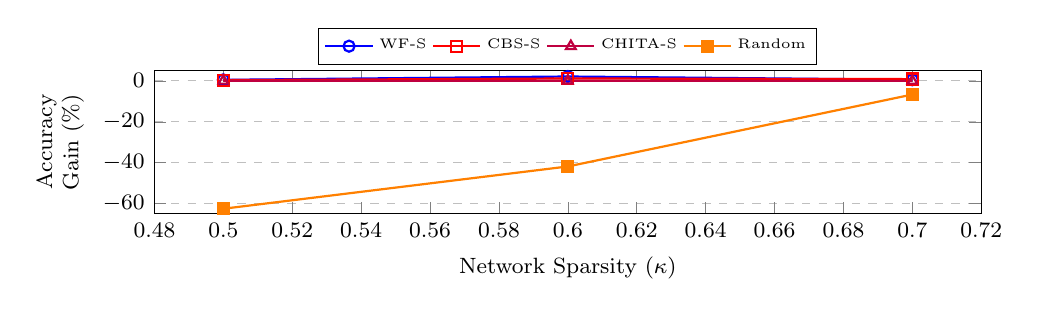
\begin{tikzpicture}
\begin{axis}[
    width=10.5cm,
    height=0.15\textwidth,
    scale only axis,
    xlabel={Network Sparsity (\(\kappa\))},
    ylabel={Accuracy \\ Gain (\%)},
    ylabel style={align=center},
    ymin=-65, ymax=5,
    ymajorgrids=true,
    grid style=dashed,
    legend pos=south east,
    legend style={
        at={(0.5,+1.3)},
        anchor=north,
        font=\tiny,
        cells={anchor=west},
        inner sep=2pt,
        legend columns=4,
    },
    tick label style={font=\footnotesize},
    label style={font=\footnotesize},
    legend cell align=left,
    mark options={scale=1},
    cycle list name=color list
]

\addplot[color=blue, mark=o, solid, thick] coordinates {
    (0.5, 0.49)
    (0.6, 2.13)
    (0.7, 0.55)
};
\addlegendentry{WF-S}

% CBS-S gain over MP
\addplot[color=red, mark=square, solid, thick] coordinates {
    (0.5, 0.35)
    (0.6, 1.16)
    (0.7, 0.85)
};
\addlegendentry{CBS-S}

% CHITA-S gain over MP
\addplot[color=purple, mark=triangle, solid, thick] coordinates {
    (0.5, 0.01)
    (0.6, 0.04)
    (0.7, 0.00)
};
\addlegendentry{CHITA-S}

\addplot[color=orange, mark=square*, solid, thick] coordinates {
    (0.5, -62.5)
    (0.6, -41.84)
    (0.7, -6.68)
};
\addlegendentry{Random}

\end{axis}
\end{tikzpicture}
\caption{Comparison of test accuracy gain over magnitude pruning for a pre-trained MobileNet (trained on ImageNet) at different sparsity levels.}
\label{fig:obs_selection}
\end{figure}


Further analysis of the similarity between pruning decisions made by MP and CHITA is provided in Appendix~\ref{appendix:pruning_similarity} to demonstrate that both methods produce nearly identical masks, underscoring the limited role of weight selection.



\subsection{Role of Hessian-Based Weight Updates}

While weight selection has negligible impact on accuracy, Hessian-based updates are critical for recovering accuracy by adjusting the remaining weights to compensate for accuracy loss due to pruning.

IP methods combine weight selection with Hessian-based updates (WF-U, CBS-U, CHITA-U). To evaluate the role of updates, we apply Hessian-based updates to MP and the resultant is denoted as MP-U. MP-U tests whether the benefits of Hessian-based updates generalize to MP's simpler selection strategy.
As shown in Figure~\ref{fig:obs_update}, MP-U achieves accuracy gains comparable to WF-U, CBS-U, and CHITA-U. This demonstrates that Hessian-based updates, not weight selection, is the primary driver of accuracy recovery. Combining Hessian-based updates with MP achieves performance on par with state-of-the-art pruning methods, eliminating the need for computationally expensive IP-selection strategies.





\begin{figure}[ht]
\centering
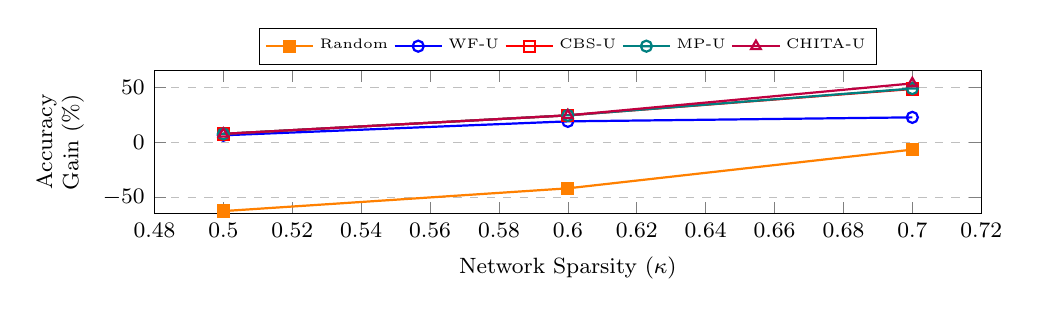
\begin{tikzpicture}
\begin{axis}[
    width=10.5cm,
    height=0.15\textwidth,
    scale only axis,
    xlabel={Network Sparsity (\(\kappa\))},
    ylabel={Accuracy \\ Gain (\%)},
    ylabel style={align=center},
    ymin=-65, ymax=65,
    ymajorgrids=true,
    grid style=dashed,
    legend pos=south east,
    legend style={
        at={(0.5,+1.3)},
        anchor=north,
        font=\tiny,
        cells={anchor=west},
        inner sep=2pt,
        legend columns=5,
    },
    tick label style={font=\footnotesize},
    label style={font=\footnotesize},
    legend cell align=left,
    mark options={scale=1},
    cycle list name=color list
]

\addplot[color=orange, mark=square*, solid, thick] coordinates {
    (0.5, -62.5)
    (0.6, -41.84)
    (0.7, -6.68)
};
\addlegendentry{Random}

\addplot[color=blue, mark=o, solid, thick] coordinates {
    (0.5, 6.3)
    (0.6, 18.96)
    (0.7, 22.58)
};
\addlegendentry{WF-U}

\addplot[color=red, mark=square, solid, thick] coordinates {
    (0.5, 7.6)
    (0.6, 24.43)
    (0.7, 48.33)
};
\addlegendentry{CBS-U}

\addplot[color=teal, mark=halfcircle, solid, thick] coordinates {
    (0.5, 7.63)
    (0.6, 24.39)
    (0.7, 48.73)
};
\addlegendentry{MP-U}


\addplot[color=purple, mark=triangle, solid, thick] coordinates {
    (0.5, 7.63)
    (0.6, 24.39)
    (0.7, 53.4)
};
\addlegendentry{CHITA-U}

\end{axis}
\end{tikzpicture}
\caption{Comparison of test accuracy gain over magnitude pruning for a pre-trained MobileNet (trained on ImageNet) at different sparsity levels.}
\label{fig:obs_update}
\end{figure}



\textbf{Insights}.
IP-selection only methods (WF-S, CBS-S, CHITA-S) offer minimal improvements over MP, confirming that weight selection has little influence on pruning performance. In contrast, Hessian-based update is the primary contributor to accuracy recovery post-pruning. These findings \textit{shift the focus from weight selection to identifying other factors affecting pruning performance}, which is explored in the next section.





